%% LyX 1.1 created this file.  For more info, see http://www.lyx.org/.
%% Do not edit unless you really know what you are doing.
\documentclass[german]{slides}
\usepackage[T1]{fontenc}
\usepackage{babel}
\usepackage[dvips]{graphics}

\makeatletter


%%%%%%%%%%%%%%%%%%%%%%%%%%%%%% LyX specific LaTeX commands.
\providecommand{\LyX}{L\kern-.1667em\lower.25em\hbox{Y}\kern-.125emX\@}

%%%%%%%%%%%%%%%%%%%%%%%%%%%%%% Textclass specific LaTeX commands.
 \newcounter{slidetype}
 \setcounter{slidetype}{0}
 \newif\ifLyXsNoCenter
 \LyXsNoCenterfalse
 \newcommand{\noslidecentering}{
    \LyXsNoCentertrue%
 }
 \newcommand{\slidecentering}{
    \LyXsNoCenterfalse%
 }
 \newcommand{\lyxendslide}[1]{
    \ifLyXsNoCenter%
         \vfill%
    \fi%
    \ifcase \value{slidetype}%
         \or % no action for 0
         \end{slide} \or%
         \end{overlay} \or%
         \end{note}%
    \fi%
    \setcounter{slidetype}{0}
	\visible
 }
 \AtEndDocument{\lyxendslide{.}}
 \newcommand{\lyxnewslide}[1]{
    \lyxendslide{.}
    \setcounter{slidetype}{1}
    \begin{slide}
 }
 \newenvironment{lyxcode}
   {\begin{list}{}{
     \setlength{\rightmargin}{\leftmargin}
     \raggedright
     \setlength{\itemsep}{0pt}
     \setlength{\parsep}{0pt}
     \verbatim@font}%
    \item[]}
   {\end{list}}

%%%%%%%%%%%%%%%%%%%%%%%%%%%%%% User specified LaTeX commands.
% Uncomment to print out only slides and overlays
%
%\onlyslides{\slides}

% Uncomment to print out only notes
%
%\onlynotes{\notes}

\usepackage{textcomp}
\makeatother

\begin{document}


\lyxnewslide{}

{\par\centering \textbf{\Large Werzeugunterst�tzung f�r die �berpr�fung der Einhaltung
von OCL-Gesch�ftsregeln in Java-Programmen}\Large \par}

{\par\centering Ralf Wiebicke\par}

{\par\centering 28. August 2000\par}


\lyxnewslide{}

{\par\centering \textbf{\Large �bersicht}\Large \par}

\vspace{10pt}\hrule height 4pt

\begin{itemize}
\item Code Injector
\item Scope von Invarianten
\item Caching von Invarianten
\item Erweiterte Typinformation in Java

\begin{itemize}
\item Statische Analyse
\item Dynamische Typverfolgung
\end{itemize}
\item Ausblick
\end{itemize}

\lyxnewslide{}

{\par\centering \textbf{\Large Code Injector - Ziele}\Large \par}

\vspace{10pt}\hrule height 4pt

\begin{itemize}
\item Ziele
\end{itemize}

\lyxnewslide{}

{\par\centering \textbf{\Large Code Injector - }\\
\textbf{\Large Probleme des einfachen Ansatzes}\Large \par}

\vspace{10pt}\hrule height 4pt

\begin{enumerate}
\item Einf�gung an jeder return-Anweisung
\item Vorberechnung des R�ckgabeausdrucks
\item Namenskonflikte
\item kompletter Javaparser notwendig
\end{enumerate}

\lyxnewslide{}

{\par\centering \textbf{\Large Code Injector - }\\
\textbf{\Large Wrapping Methods}\Large \par}

\vspace{10pt}\hrule height 4pt

\begin{lyxcode}
int~someMethod(double~x)~\\
\{~\\
~~//~here~comes~the~code.~\\
\}~
\end{lyxcode}
\vspace{10pt}\hrule height 1pt

\begin{lyxcode}
int~someMethod\_wrappedbyocl(double~x)~\\
\{~\\
~~//~here~comes~the~code.~\\
\}~\\
~~\\
int~someMethod(double~x)~\\
\{~\\
~~//~pre~method~code~\\
~~int~result=someMethod\_wrappedbyocl(x);~\\
~~//~post~method~code~\\
~~return~result;~\\
\}
\end{lyxcode}

\lyxnewslide{}

{\par\centering \textbf{\Large Code Injector - }\\
\textbf{\Large Wrapping Constructors}\Large \par}

\vspace{10pt}\hrule height 4pt

\begin{lyxcode}
SomeClass(String~x)~\\
\{~\\
~~//~here~comes~the~code~\\
\}
\end{lyxcode}
\vspace{10pt}\hrule height 1pt

\begin{lyxcode}
SomeClass(String~x,~Dummy)~\\
\{~\\
~~//~here~comes~the~code~\\
\}~\\
~~\\
SomeClass(String~x)~\\
\{~\\
~~this(x,~(Dummy)null);~\\
~~//~post~constructor~code~\\
\}
\end{lyxcode}

\lyxnewslide{}

{\par\centering \textbf{\Large Scope von Invarianten}\Large \par}

\vspace{10pt}\hrule height 4pt

Wann m�ssen die Invarianten erf�llt sein?

\begin{itemize}
\item Alle Methoden.
\item �ffentliche Methoden.
\item Ausgezeichnete Methoden.
\item Explizite Pr�fung.
\end{itemize}

\lyxnewslide{}

{\par\centering \textbf{\Large Caching von Invarianten}\Large \par}

\vspace{10pt}\hrule height 4pt

\vspace{0.3cm}
{\par\centering \resizebox*{1\textwidth}{!}{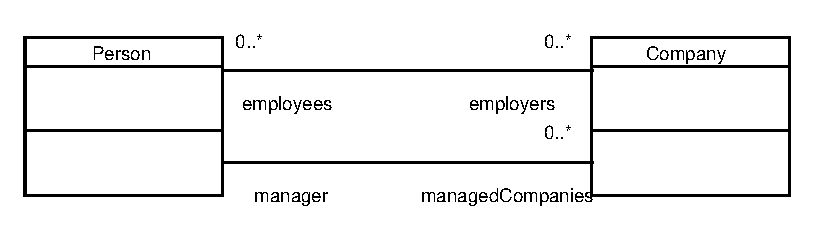
\includegraphics{PersonCompany.eps}} \par}
\vspace{0.3cm}

\begin{lyxcode}
context~Company~inv:~\\
~~manager.age>=0~\\
~\\
context~Company~inv:~\\
~~employees.age>=0~\\
~\\
context~Company~inv:~\\
~~employees.getAge()>=0~\\
~\\
context~Company~inv:~\\
~~employees.getIncomeAfterTax(0.15)>=5000
\end{lyxcode}

\lyxnewslide{}

{\par\centering \textbf{\Large �berwachung von Attributen}\Large \par}

\vspace{10pt}\hrule height 4pt

\begin{lyxcode}
class~Person~\\
\{~\\
~~int~age;~\\
~~int~age\_oclbackup=age;~\\
~~\\
~~private~void~checkForChangedFeatures()~\\
~~\{~\\
~~~~if(age!=age\_oclbackup)~\\
~~~~\{~\\
~~~~~~age\_oclbackup=age;~\\
~~~~~~//~notify~observers~of~age~\\
~~~~\}~\\
~~~~//~...~further~attributes~\\
~~\}~\\
\}
\end{lyxcode}

\lyxnewslide{}

{\par\centering \textbf{\Large Ausblick}\Large \par}

\vspace{10pt}\hrule height 4pt

\begin{itemize}
\item Typechecker for observed
\item Observe Methods
\item Application Netlinx
\item tagged Methods scope
\end{itemize}
\end{document}
